Toda la información de los clientes del segmento \textbf{Corporate} que realizaron una orden con modo de envío \textbf{First Class}
y que no viven en \textbf{California}. \\

En primera instancia, \textit{seleccionamos} los clientes que pertenecen al segmento \textbf{Corporate} y que no viven en \textbf{California} de la relación \textit{customer}, almacenando dichas tuplas en una relación temporal \textit{r} . Luego, seleccionamos las órdenes cuyo modo de envío es \textbf{First Class} de la relación \textit{orders}. Finalmente, realizamos un natural join entre las dos relaciones resultantes para obtener lo que nos pide el inciso. \\

\begin{center}
    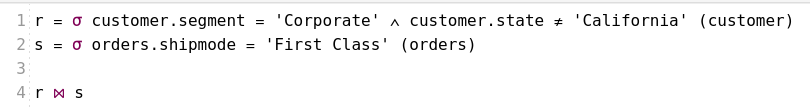
\includegraphics[width=14cm]{resources/pregunta2/2.4.1.png} \\
\end{center}

Ahora el arbol de la consulta se ve de la siguiente manera: \\

\begin{center}
    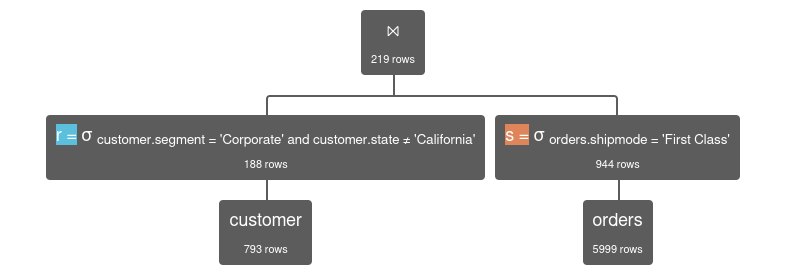
\includegraphics[width=14cm]{resources/pregunta2/2.4.2.png} \\
\end{center}

y parte de la tabla resultante es la siguiente: \\
\begin{center}
    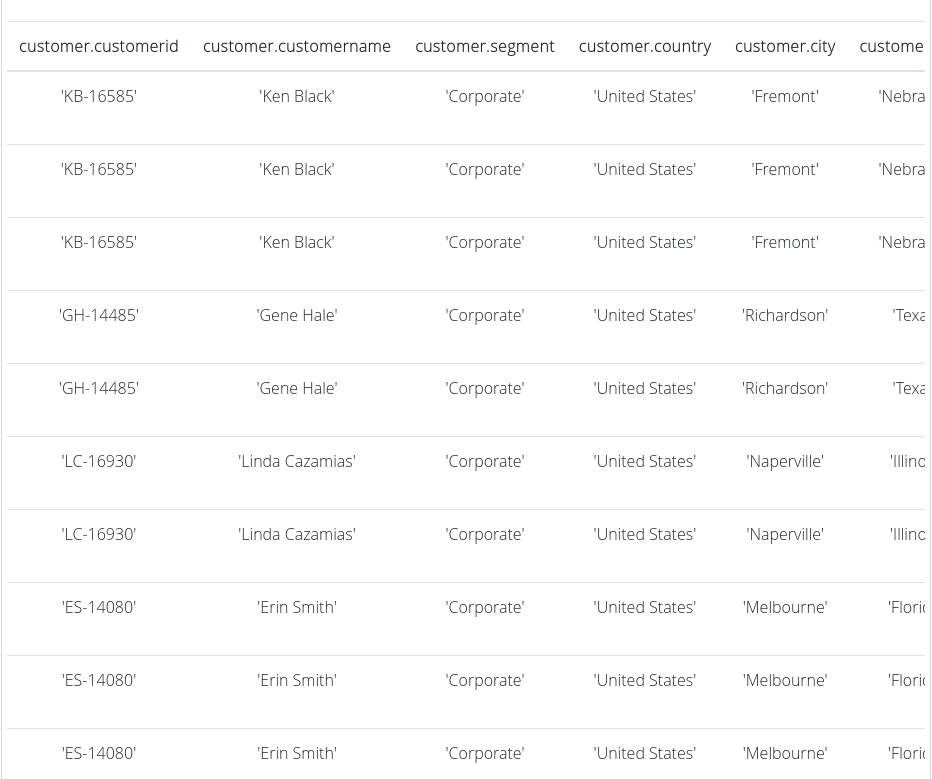
\includegraphics[width=10cm]{resources/pregunta2/2.4.3.png} \\
\end{center}

\begin{center}  
    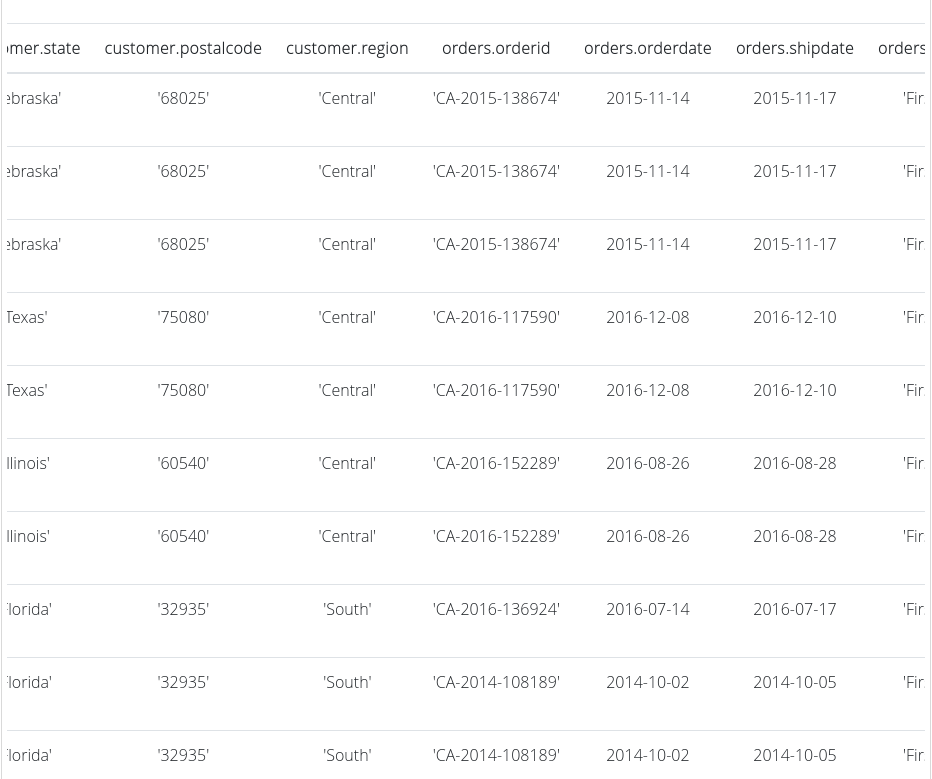
\includegraphics[width=10cm]{resources/pregunta2/2.4.4.png} \\
\end{center}
    